% !TEX TS-program = pdflatex
% !TEX encoding = UTF-8 Unicode

% This is a simple template for a LaTeX document using the "article" class.
% See "book", "report", "letter" for other types of document.

\documentclass[11pt]{article} % use larger type; default would be 10pt

\usepackage[utf8]{inputenc} % set input encoding (not needed with XeLaTeX)

%%% Examples of Article customizations
% These packages are optional, depending whether you want the features they provide.
% See the LaTeX Companion or other references for full information.

%%% PAGE DIMENSIONS
\usepackage{geometry} % to change the page dimensions
\geometry{a4paper} % or letterpaper (US) or a5paper or....
% \geometry{margin=2in} % for example, change the margins to 2 inches all round
% \geometry{landscape} % set up the page for landscape
%   read geometry.pdf for detailed page layout information

\usepackage{graphicx} % support the \includegraphics command and options

% \usepackage[parfill]{parskip} % Activate to begin paragraphs with an empty line rather than an indent

%%% PACKAGES
\usepackage{booktabs} % for much better looking tables
\usepackage{array} % for better arrays (eg matrices) in maths
\usepackage{paralist} % very flexible & customisable lists (eg. enumerate/itemize, etc.)
\usepackage{verbatim} % adds environment for commenting out blocks of text & for better verbatim
\usepackage{subfig} % make it possible to include more than one captioned figure/table in a single float
\usepackage{amsmath}
\usepackage{mathtools}
\usepackage[thinc]{esdiff}
% These packages are all incorporated in the memoir class to one degree or another...

%%% HEADERS & FOOTERS
\usepackage{fancyhdr} % This should be set AFTER setting up the page geometry
\pagestyle{fancy} % options: empty , plain , fancy
\renewcommand{\headrulewidth}{0pt} % customise the layout...
\lhead{}\chead{}\rhead{}
\lfoot{}\cfoot{\thepage}\rfoot{}

%%% SECTION TITLE APPEARANCE
\usepackage{sectsty}
\allsectionsfont{\sffamily\mdseries\upshape} % (See the fntguide.pdf for font help)
% (This matches ConTeXt defaults)

%%% ToC (table of contents) APPEARANCE
\usepackage[nottoc,notlof,notlot]{tocbibind} % Put the bibliography in the ToC
\usepackage[titles,subfigure]{tocloft} % Alter the style of the Table of Contents
\renewcommand{\cftsecfont}{\rmfamily\mdseries\upshape}
\renewcommand{\cftsecpagefont}{\rmfamily\mdseries\upshape} % No bold!

%%% END Article customizations

%%% The "real" document content comes below...

\title{Distribution}
\author{Mingwei Fei}
%\date{} % Activate to display a given date or no date (if empty),
         % otherwise the current date is printed 

\begin{document}
\maketitle

\section{Distribution Transformation}
Let $X \sim Gamma(\alpha, 1)$ and $Y \sim Gamma(\beta, 1)$ where the paramaterization is such that $\alpha$ is the shape parameter. Then 
\begin{align*}
	\frac{X}{X+Y} \sim Beta(\alpha, \beta)
\end{align*}

\begin{itemize}
	\item [(i)] How do we create the transformed variables $U= \frac{X}{X+Y} $, V, such that it is easy to get the distribution of U and V, and easy to integrate out V to get the margin distribution of U? This requires familiarity of Beta and Gamma distribution.
	
	One proposal is $V= Y$, and the other is $V= X+Y$. Compare between the two and see which one is better.
	
	\textbf{Note:} The way to choose new parameter is easier to get the original parameter by simple arithmetic calculation or just itself.
	If we are using the first set of new parameter, it would get the distribution very complicated, the Beta distribution has the form of $U, 1-U$, need to keep in mind of the achieving the product of two distribution form. 
	
	
	
	\item[(ii)] We could see that $V=X+Y$ is better as U and V are independent from each other.
\begin{align*}
	f(X) &= \frac{1}{\Gamma{(\alpha)}} x^{\alpha-1} e^{-x}\\
	f(Y) &= \frac{1}{\Gamma{(\beta)}} y^{\beta-1} e^{-y}
\end{align*}	
Let
\begin{align*}
	U &= \frac{X}{X+Y}, \qquad V = X + Y
\end{align*}	
Then
\begin{align*}
	X &= UV, \qquad Y = V - UV
\end{align*}
	 	
The Jacobian transformation matrix
\begin{align*}
	J &= \begin{pmatrix}
		\diffp{X}{U} & \diffp{X}{V} \\
		\diffp{Y}{U} & \diffp{Y}{V} 
	\end{pmatrix} =  \begin{pmatrix}
	V & U \\
	-V & 1-U
\end{pmatrix}\\
|J| &= V
\end{align*}
X and Y are independent, so the joint distribution of (X, Y) 
\begin{align*}
	f(X, Y) &= \frac{1}{\Gamma{(\alpha)} \Gamma{(\beta)}} x^{\alpha -1} e^{-x} y^{\beta -1} e^{-y}\\
	f(U, V) &= \frac{1}{\Gamma{(\alpha)} \Gamma{(\beta)}} U^{\alpha -1} (1-U)^{\beta -1} V^{\alpha + \beta -1} e^{-V}
\end{align*}

We don't always need to integrate out the other parameter, if we can write the distribution in the form that we can recognize, then will directly get the distribution. 

$V \sim Gamma (\alpha + \beta, 1)$ and $U \sim Beta(\alpha, \beta)$.

\end{itemize}



\subsection{Gamma distribution and Beta distribution}
If $Y_1, ..., Y_{n+1}$ are i.i.d $Exp(\theta)$, then 
\begin{align*}
	Z_i &= \frac{Y_1 + ...+ Y_i}{Y_1+ .. + Y_{n+1}} \sim Beta(i, n-i+1) 
\end{align*}
Particularly, $(Z_1, ... Z_n)$ has the same distribution as the order statistics $(\xi_{n:1}, .. \xi_{n:n})$ of n Uniform(0,1) random variables.

\subsubsection{Prove Beta distribution}
The $Z_{n+1} = 1$, so we don't need to calculate this distribution. 
We can use the method in above problem to get the distribution of $Z_i$, and we need to get the joint distribution of $(Z_1, ... Z_n)$.

Let 
\begin{align*}
	U &=Y_1 + ...+ Y_i, \qquad V= Y_{i+1}+ .. + Y_{n+1} 
\end{align*}
Then $U \sim Gamma(i, \theta), V \sim Gamma(n+1-i, \theta)$, Let
\begin{align*}
 	Z_i &= U/(U+V), \qquad W = U+V 
\end{align*}

Consider the transformation $(U,V)^T \rightarrow (Z_i, W)^T$, note that the transform is one-to-one with the Jacobian
\begin{align*}
	\Bigg |\diffp{(U,V)}{{(Z_i, W)}} \Bigg | &= |W|
\end{align*}
 
For joint distribution of  $(U,V)^T$, 
\begin{align*}
	\frac{1}{\Gamma{(i)}} \theta exp(-\theta u) (\theta u)^{i-1} I(u > 0) \times \frac{1}{\Gamma{(n+1-i)}} \theta exp(-\theta v) (\theta v)^{n-i} I(v > 0)
\end{align*}
We obtain the joint density of $(Z_i, W)$ as 
\begin{align*}
&	\frac{1}{\Gamma{(i)}} \theta exp(-\theta z_i w) (\theta z_i w)^{i-1} \\
	& \times \frac{1}{\Gamma{(n+1-i)}} \theta exp(-\theta (1-z_i) w) (\theta (1-z_i) w)^{n-i} w \times I(0< z_i< 1) I(w > 0)
\end{align*}

Thus, the marginal density of $Z_i = X/(X+Y)$ is equal to
\begin{align*}
 & (1-z_i)^{n-i} z_i^{i-1} I(0< z_i <1)	\frac{\Gamma(n+1)}{\Gamma(i) \Gamma(n+1-i)} \int_{w} \theta exp(-\theta w) (\theta w)^n I(w>0) 	dw \\
 &= \frac{\Gamma(n+1)}{\Gamma(i) \Gamma(n+1-i)} (1-z_i)^{n-i} z_i^{i-1} I(0< z_i <1)
\end{align*}
That is $Z_i \sim Beta(i, n+1-i)$

\subsubsection{Prove Uniform distribution}



We need to note that, we always construct a joint distribution as we are using the $Y_1, ..., Y_{n+1}$ in joint distribution. So the transformed variables are also joint distribution.

Then we need to find the relationship between $Y_1, ..., Y_{n+1}$ and $(Z_1, ... Z_n)$. We can set the total sum as $S_{n+1} = Y_1+ .. + Y_{n+1}$.

\begin{align*}
	Y_1 &= Z_1 \times S_{n+1} \\
	Y_2 &= Z_2 \times S_{n+1} - Y_1 = (Z_2  - Z_1) \times S_{n+1}\\
	Y_3 &= Z_3 \times S_{n+1} - Y_1 - Y_2 = (Z_3  - Z_2) \times S_{n+1}\\
	.. & ..\\
	Y_n &= Z_n \times S_{n+1} - Y_1 - ...- Y_{n-1} = (Z_n  - Z_{n-1}) \times S_{n+1}\\
	Y_{n+1} &= S_{n+1} - Y_1 - ...- Y_{n} = (1- Z_n)  \times S_{n+1}
\end{align*}
Then we have the Jacobian transform distribution
\begin{align*}
	J &= \begin{pmatrix}
		\diffp{Y_1}{{Z_1}} & \diffp{Y_1}{{Z_2}} ... & \diffp{Y_1}{{Z_n}} & \diffp{Y_1}{{S_{n+1}}}\\
		..& ..& ..& ..\\
		\diffp{Y_n}{{Z_1}} & \diffp{Y_n}{{Z_2}}  ... & \diffp{Y_n}{{Z_n}} & \diffp{Y_n}{{S_{n+1}}}\\
		\diffp{Y_{n+1}}{{Z_1}} & \diffp{Y_{n+1}}{{Z_2}} & ...& \diffp{Y_{n+1}}{{S_{n+1}}}
	\end{pmatrix} =  \begin{pmatrix}
		S_{n+1} & 0 & 0 &.. & ..& Z_1  \\
		-S_{n+1} & S_{n+1} & 0 &.. &..& Z_2- Z_1  \\
		.. & .. & .. \\
		0 & 0&.. -S_{n+1} & S_{n+1}  &0 & Z_{n}- Z_{n-1}  \\
		0 & 0 &..& 0 & S_{n+1}& 1- Z_n\\
	\end{pmatrix}\\
	|J| &= S_{n+1}^{n}
\end{align*}

The joint distribution of $Y_1, ..., Y_{n+1}$
\begin{align*}
	f(Y_1, Y_2,.. Y_{n+1}) &= \prod_{i=1}^{n+1} \frac{1}{\theta} exp(-\frac{y_i}{\theta}) I(0< y_i < \infty) \\
	&= \frac{1}{\theta^{n+1}} exp(-\frac{\sum_{i=1}^{n+1} y_i}{\theta}) I(0< y_i < \infty)\\
	&= \frac{1}{\theta^{n+1}} exp(-\frac{S_{n+1}}{\theta}) I(0< y_i < \infty)
\end{align*}

Then the transformed variables
\begin{align*}
	f(Z_1, Z_2,.. Z_{n}, S_{n+1}) &= \frac{1}{\theta^{n+1}} exp(-\frac{S_{n+1}}{\theta}) S_{n+1}^{n} I(0< z_1 < z_2 <.. <z_n < 1) I(S_{n+1} > 0)
\end{align*}

We obtain the joint distribution of $(Z_1, ... Z_n)$

\begin{align*}
	f(Z_1, Z_2,.. Z_{n}) &= \int_{s} f(Z_1, Z_2,.. Z_{n}, S_{n+1}) dS \\
	&= \int_{s} \frac{1}{\theta^{n+1}} exp(-\frac{S}{\theta}) S^{n} I(0< z_1 < z_2 <.. <z_n < 1) I(S > 0) dS\\
	&= n! I(0< z_1 < z_2 <.. <z_n < 1), \qquad \text{Gamma integral}
\end{align*}
which is the joint density of order statistics of n uniform (0,1) random variables.

\begin{figure}
	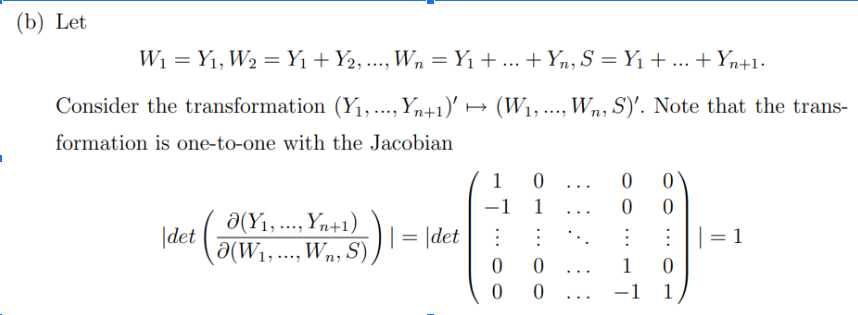
\includegraphics[width=15cm]{Figure/dist1.PNG}  
	\caption{Alt method}
\end{figure}
\begin{figure}
	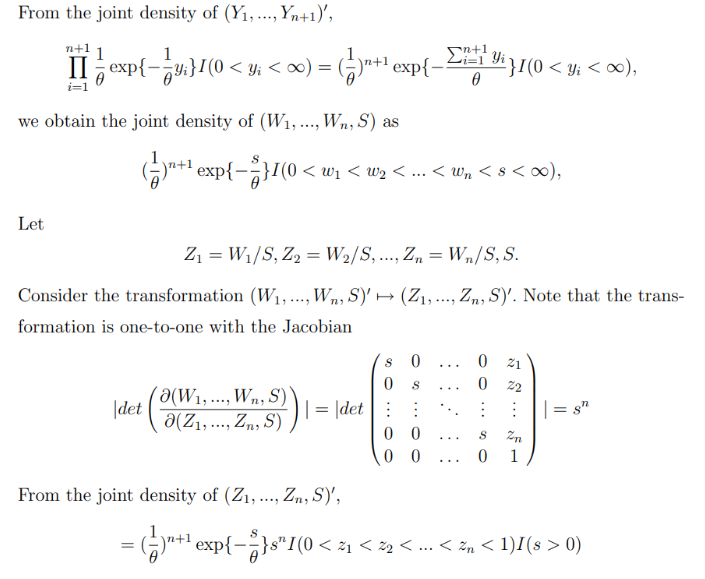
\includegraphics[width=20cm]{Figure/dist2.PNG}  
	\caption{Alt method 2}
\end{figure}





\section{Moment Generating Function}
We can get MGF from $E[x^2 t]$
\begin{align*}
	M_i(t) &= E[x^2 t] = \frac{1}{\sqrt{2\pi}} \int exp(x^2 t) exp \left( - \frac{(x-\mu)^2}{2} \right) dx\\
	&=  \frac{1}{\sqrt{2\pi}}  \int exp \left( (t- \frac{1}{2}) x^2 + \mu x -\frac{\mu^2}{2} \right) dx \\
	&=  \frac{1}{\sqrt{2\pi}}  \int exp \left(  -\frac{1}{2}(1-2t) \{ x^2 - \frac{2 \mu x}{(1-2t)} + \frac{\mu^2}{(1-2t)^2} \} + \frac{\mu^2}{2(1-2t)} -\frac{\mu^2}{2}  \right) dx \\
	&= \frac{1}{\sqrt{(1-2t)}} \int \frac{(1-2t)}{\sqrt{2\pi}} exp\left( -\frac{(x-\frac{\mu}{1-2t})^2}{2 (1-2t)^{-1}} \right) dx \left[exp \left( \frac{\mu^2 t}{1-2t} \right) \right]\\
	&=\frac{1}{\sqrt{(1-2t)}} exp \left( \frac{\mu^2 t}{1-2t} \right), \qquad \lambda = \mu^2\\
	&=\frac{1}{\sqrt{(1-2t)}} exp \left( \frac{\lambda t}{1-2t} \right)
\end{align*}

Then the MGF for $Q_i \sim \chi^2 _{k_i}(\lambda_i)$
\begin{align*}
	M(t) &= E[ \sum_{i=1}^k x_i^2 t] = \prod_{i=1}^k M_i(t) \\
	&=\left(\frac{1}{\sqrt{(1-2t)}} \right)^k exp \left( \frac{ \sum_{i=1}^k \lambda_i t }{1-2t} \right)\\
	&=\left(\frac{1}{\sqrt{(1-2t)}} \right)^k exp \left( \frac{ \lambda t }{1-2t} \right)\\
	&= (1-2t)^{-k/2} exp \left( \frac{ \lambda t }{1-2t} \right), \qquad \text{i.i.d}
\end{align*}

The general case of a linear combination of independent $\chi^2_{k_i}(\lambda_i)$

\begin{align*}
	Q &= \sum_{i=1}^k a_i Q_i
\end{align*}
We also can prove using MGF.

\subsubsection{Linear Combination of Chi-Square Distribution}
The linear combination of chi-square distribution $Y_j$. Let us denote by $X \sim \Gamma(r, \lambda)$ the fact that the r.v. X has a Gamma distribution with shape parameter r and rate parameter $\lambda$ 

\begin{align*}
	f_{X}(x) &= \frac{\lambda^x}{\Gamma (r)} exp(- \lambda x) x^{r-1}, \qquad (r, \lambda >0, x >0)
\end{align*}

Then we have, for $j=1,..p$,

\begin{align*}
	Y_j & \sim  \Gamma(\frac{k_j}{2}, \frac{1}{2}) \rightarrow Z_j = w_j Y_j \sim \Gamma(\frac{k_j}{2}, \frac{1}{2w_j})
\end{align*}

The MGF for linear combinations $Z_j = w_j Y_j$
\begin{align*}
	M(t) &= E[exp(Y_j t)] = (1-2t)^{-k/2} exp \left( \frac{ \lambda t }{1-2t} \right)\\
	M_{Z_j} (t) & = E[exp(w_j Y_j t)] = E[exp( Y_j (w_jt))] \\
	&= (1-2 w_jt)^{-1/2} exp \left( \frac{ \lambda w_j t }{1-2 w_j t} \right)
\end{align*}

\begin{align*}
	M_Y(t) &= E[exp(Y t)] = E[exp(t [w_1 Y_1 + w_2 Y_2 + w_3 Y_3 +.. w_n Y_n])]\\
	&= E[exp(w_1 t Y_1)]E[exp(w_2 t Y_2)]... E[exp(w_n t Y_n)]\\
	&= M_{X_1}(w_1 t) M_{X_2}(w_2 t) M_{X_3}(w_3 t).. M_{X_n}(w_n t)\\
	&= \prod_{i=1}^n M_{X_i}(w_i t)
\end{align*}

The third equation comes from the properties of exponents, as wells as from the expectation of the product of functions of independent random variables. 

I need to pay attention that, only under independent and identical situation, we can write
 \begin{align*}
 	M_Y(t) &= M_{X}(t)^n
 \end{align*}

Other than that, we can not further simplify that. So back to the non-central chi-square distribution, we have the MGF of Y
\begin{align*}
	M_Y(t) &= \prod_{i=1}^n M_{X_i}(w_i t)\\
	&=\prod_{i=1}^n  (1-2 w_jt)^{-1/2} exp \left( \frac{ \lambda w_j t }{1-2 w_j t} \right)
\end{align*}

Then we can see that the shape parameter is $\frac{1}{2 w_i}$. If we want to have a non-central chi-square distribution for $Y$, then all $w_j$ need to be the same. 


\subsection{b}Consider the following
\begin{itemize}
	\item[(a)] For an arbitrary model, consider the conditional score statistic
	\begin{align*}
		U_{\psi}(\xi) &= \frac{\partial l_c(\xi, \psi_0)}{\partial \psi} |_{\psi_0=\psi}
	\end{align*} 
	Show that the conditional score statistic for any model can be written as
	\begin{align*}
		U_{\psi}(\xi) &= \partial_{\psi} log p(Y|\xi)- E[\partial_{\psi} log p(Y|\xi)|s_{\lambda}(\psi_0)]|_{\psi_0=\psi}
	\end{align*} 
	The conditional score statistic is the derivative of the conditional distribution
	\begin{align*}
		U_{\psi}(\xi) &= \frac{\partial l_c(\xi, \psi_0)}{\partial \psi} |_{\psi_0=\psi}\\
		p(\textbf{Y}| \xi) &= p(\textbf{Y}|s_{\lambda}(\psi_0), \xi) p(s_{\lambda}(\psi_0) | \xi), \qquad p(\textbf{Y}|s_{\lambda}(\psi_0), \xi) = \frac{p(\textbf{Y}| \xi)}{p(s_{\lambda}(\psi_0) | \xi)} \\
		l_c(\xi, \psi_0) &= log p(\textbf{Y}|s_{\lambda}(\psi_0), \xi)= log p(\textbf{Y}| \xi) - log p(s_{\lambda}(\psi_0) | \xi)
	\end{align*}
	Then we need to prove 
	\begin{align*}
		U_{\psi}(\xi) &= \frac{\partial l_c(\xi, \psi_0)}{\partial \psi} |_{\psi_0=\psi} = \partial_{\psi} log p(\textbf{Y}| \xi) - \partial_{\psi} log p(s_{\lambda}(\psi_0) | \xi)\\
		\partial_{\psi} log p(s_{\lambda}(\psi_0) | \xi) &= E[\partial_{\psi} log p(Y|\xi)|s_{\lambda}(\psi_0)]|_{\psi_0=\psi}
	\end{align*}
	We can write
	\begin{align*}
		log p(\textbf{Y}| \xi) &= log  p(\textbf{Y}|s_{\lambda}(\psi_0), \xi) + log p(s_{\lambda}(\psi_0) | \xi)\\
		E \left( \partial_{\psi}[log p(\textbf{Y}| \xi)| s_{\lambda}]\right) &= E \left(\partial_{\psi}[log  p(\textbf{Y}|s_{\lambda}(\psi_0), \xi)|s_{\lambda}]\right) + E \left(\partial_{\psi}[log p(s_{\lambda}(\psi_0), \xi)|s_{\lambda}]\right)
	\end{align*}    
	in which, the integral and expectation can switch, then we have
	\begin{align*}
		E \left(\partial_{\psi}[log  p(\textbf{Y}|s_{\lambda}(\psi_0), \xi)|s_{\lambda}]\right) & = \partial_{\psi} E \left([log  p(\textbf{Y}|s_{\lambda}(\psi_0), \xi)|s_{\lambda}]\right) = \partial_{\psi} E \left([log  p(\textbf{Y}| \xi)]\right)= 0
	\end{align*}      
	So,
	\begin{align*}
		E \left( \partial_{\psi}[log p(\textbf{Y}| \xi)| s_{\lambda}]\right) &= \partial_{\psi}log p(s_{\lambda}(\psi_0),\xi)
	\end{align*}
	Then we show
	\begin{align*}
		U_{\psi}(\xi) &= \partial_{\psi} log p(Y|\xi)- E[\partial_{\psi} log p(Y|\xi)|s_{\lambda}(\psi_0)]|_{\psi_0=\psi}
	\end{align*} 
	\item[(b)] Suppose that $y_1;.. y_n$ are independent and $y_i$ follows a Poisson distribution with mean $exp(\lambda_0 + \lambda_1x_{i1} +  \psi x_{i2})$, where $(x_{i1}; x_{i2})$ are covariates, $\lambda = (\lambda_0; \lambda_1)$ is the
	nuisance parameter vector and $\psi$  is the parameter of interest. Derive the conditional
	likelihood of $\psi$   and show that this conditional likelihood is free of $\lambda$.\\
	The joint distribution of $(y_1, · · · , y_n)$ is given by 
	\begin{align*}
		P(Y|\lambda, \psi)&=  exp \left( \sum_{i=1}^n y_i(\lambda_0 + \lambda_1x_{i1} +  \psi x_{i2}) - \sum_{i=1}^n exp(\lambda_0 + \lambda_1x_{i1} +  \psi x_{i2}) - log y_i! \right)
	\end{align*}
	Thus, $S_0 = \sum_{i=1}^n y_i$ is the sufficient and complete statistics for $\lambda_0$, and $S_1 = \sum_{i=1}^n y_i x_{i1}$ is the sufficient and complete statistics for $\lambda_1$.\\
	The conditional distribution of $\psi$ given $S_0, S_1$ is given by
	\begin{align*}
		p(\textbf{Y}, \psi|S=(S_0, S_1)) &= \frac{exp \left( \sum_{i=1}^n y_i(\lambda_0 + \lambda_1x_{i1} +  \psi x_{i2}) - \sum_{i=1}^n exp(\lambda_0 + \lambda_1x_{i1} +  \psi x_{i2}) - log y_i! \right)}{\sum_{y' \in S} exp \left( \sum_{i=1}^n y'_i(\lambda_0 + \lambda_1 x_{i1} +  \psi x_{i2}) - \sum_{i=1}^n exp(\lambda_0 + \lambda_1 x_{i1} +  \psi x_{i2}) - log y'_i! \right)}\\
		&= \frac{exp \left( S_1 \lambda_0 + S_2 \lambda_1 +  S_3 \psi) - \sum_{i=1}^n exp(\lambda_0 + \lambda_1x_{i1} +  \psi x_{i2}) - log y_i! \right)}{\sum_{y' \in S} exp \left( S'_1\lambda_0 + S'_2 \lambda_1 + S'_3 \psi) - \sum_{i=1}^n exp(\lambda_0 + \lambda_1 x_{i1} +  \psi x_{i2}) - log y'_i!\right)} \\
		&= \frac{exp \left( S_3 \psi  - log y_i!\right)}{\sum_{y' \in S} exp \left( S'_3 \psi - log y'_i! \right)}, \qquad S_3 = \sum_{i=1}^n y_i x_{i2}, S'_3 = \sum_{i=1}^n y'_i x_{i2}
	\end{align*}
	which is independent of $\lambda$. \\
	\item[(c)] Derive the conditional score statistic for part (b) and write out a Newton-Raphson algorithm for obtaining the conditional maximum likelihood estimate of $\psi$  based on $U_{\psi}(\xi)$.\\
	The log likelihood of the conditional distribution is
	\begin{align*}
		l_c(\psi) &= S_3 \psi  - log y_i! -log \left[ \sum_{y' \in S} exp \left( S'_3 \psi - log y'_i! \right) \right], \qquad S_3 = \sum_{i=1}^n y_i x_{i2}, S'_3 = \sum_{i=1}^n y'_i x_{i2}
	\end{align*} 
	The score function and observed fisher information is
	\begin{align*}
		U_{\psi}(\xi) &= \frac{\partial l_c(\xi, \psi_0)}{\partial \psi} |_{\psi_0=\psi}\\
		&= \psi - \frac{\sum_{y' \in S} S'_3 exp \left( S'_3 \psi - log y'_i! \right)}{\sum_{y' \in S} exp \left( S'_3 \psi - log y'_i! \right)}\\
		\frac{\partial^2 l_c(\xi, \psi_0)}{\partial \psi^2} &= \left[ \frac{\sum_{y' \in S} S'_3 exp \left( S'_3 \psi - log y'_i! \right)}{\sum_{y' \in S} exp \left( S'_3 \psi - log y'_i! \right)}\right]^2 - \frac{\sum_{y' \in S} S'^2_3 exp \left( S'_3 \psi - log y'_i! \right)}{\sum_{y' \in S} exp \left( S'_3 \psi - log y'_i! \right)}
	\end{align*}
	The newton-Raphson algorithm
	\begin{align*}
		\psi^{k+1} &= \psi^{k} - \left[\frac{\partial^2 l_c(\psi^{k})}{\partial \psi^2} \right]^{-1} U_{\psi}(\psi^{k})
	\end{align*}
	where $\frac{\partial^2 l_c(\psi^{k})}{\partial \psi^2}, U_{\psi}(\psi^{k})$ are from above equations.
	
	\item[(d)] Now suppose that we only have two random variables $y_1 \sim Poisson(\mu_1)$ and $y_2 \sim
	Poisson(\mu_2)$, where $y_1$ and $y_2$ are independent. We are interested in making inferences on the ratio $\psi = \mu_1/\mu_2$. Let $\xi = (\psi , \lambda)$, where $\lambda$ represents the nuisance parameter.
	\begin{itemize}
		\item [(i)] Show that the log-likelihood function of $\xi$ can be written as
		\begin{align*}
			l(\xi) &= (y_1 + y_2)\lambda + y_1 log (\psi) - exp(\lambda) (1+\psi)
		\end{align*}
		where $\lambda$ is a function of $\mu_2$. Explicitly state what $\lambda$ is.\\
		Write the joint distribution of $y_1, y_2$
		\begin{align*}
			P(y_1, y_2) &= \frac{\mu_1^{y_1} e^{-\mu_1}}{y_1!} \frac{\mu_2^{y_2} e^{-\mu_2}}{y_2!} \\
			log P(y_1, y_2) &= y_1 log \mu_1 - \mu_1 + y_2 \log \mu_2 - \mu_2 - log y_1! - log y_2!\\
			&= y_1 log \frac{\mu_1}{\mu_2} + y_1 log \mu_2 + y_2 log \mu_2 -\mu_1 - \mu_2 -log y_1! - log y_2!\\
			&= y_1 log \frac{\mu_1}{\mu_2} + (y_1+y_2) log \mu_2 - \mu_2(\mu_1/\mu_2 + 1) -log y_1! - log y_2!
		\end{align*}
		where 
		\begin{align*}
			\psi &=log \frac{\mu_1}{\mu_2} \\
			\lambda &= log \mu_2
		\end{align*}
		\item[(ii)] Derive the conditional likelihood of $\psi$  and write out a Newton-Raphson algorithm for obtaining the conditional maximum likelihood estimate of $\psi$ .\\
		From part (a), we see $y_1 + y_2$ is the sufficient statistics for $\lambda$, while $y_1 + y_2 \sim Poission (\mu_1+\mu_2)$ then we have conditional distribution of $\psi$ condition on $S = y_1 + y_2$.
		\begin{align*}
			Y(\psi|S= y_1+y_2,\lambda) &= \frac{exp \left[ y_1 \psi + (y_1+y_2) \lambda - exp(\lambda)(\psi + 1) -log y_1! - log y_2! \right] }{exp \left[ (y_1+y_2) log (\mu_1+\mu_2) - (\mu_1+\mu_2) -log (y_1+y_2)!  \right]}\\
			&= \frac{exp \left[ y_1 \psi + S \lambda - exp(\lambda)(\psi + 1) -log y_1! - log y_2! \right] }{exp \left[ S (\lambda + log(\psi + 1)) -  exp(\lambda)(\psi + 1) -log S!  \right]}\\
			&= \frac{exp \left[ y_1 \psi -log y_1! - log y_2! \right] }{exp \left[ (y_1+ S-y_1) log(\psi + 1)) -log S!  \right]}\\
			&= {S \choose y_1} \left( \frac{\psi}{1+\psi}\right)^{y_1} \left(\frac{1}{1+\psi} \right)^{S-y_1}
		\end{align*}
		The conditional distribution is a binomial, $B(S, \psi/(1+\psi))$.\\
		The score function and observed fisher information 
		\begin{align*}
			log Y(\psi|S,\lambda) &= y_1 log \psi -S log(1+\psi) + log {S \choose y_1} \\
			\partial_{\psi} log Y(\psi|S,\lambda) &= \frac{y_1}{\psi} - \frac{S}{1+\psi} = 0, \qquad \hat{\psi} = y_1/(S-y_1)\\
			\partial^2_{\psi} log Y(\psi|S,\lambda) &= -\frac{y_1}{\psi^2} + \frac{S}{(1+\psi)^2}
		\end{align*}
		The $CMLE = \hat{\psi} = y_1/(S-y_1)$. And the newton-Raphson equation 
		\begin{align*}
			\psi^{k+1} &= \psi^{k} - \left[\frac{\partial^2 l_c(\psi^{k})}{\partial \psi^2} \right]^{-1} U_{\psi}(\psi^{k})\\
			&= \psi^{k} - \left[ -\frac{y_1}{\psi^2} + \frac{S}{(1+\psi)^2}\right]^{-1} \left[\frac{y_1}{\psi} - \frac{S}{1+\psi} \right]|_{\psi = \psi^{k}}\\
			&=  \psi^{k} + \frac{y_1/\psi^{k} - S/(1+\psi^{k})}{y_1/{\psi^{k}}^2 - S/(1+\psi^{k})^2}
		\end{align*}
	\end{itemize}
\end{itemize}



\end{document}
